\part{GLib, la biblioteca principal\label{glib}}

\chapter{GLib, la biblioteca principal}

GLib es la biblioteca central de bajo nivel que forma la base para proyectos como GTK y GNOME. Proporciona estructuras de datos, funciones de utilidad, envoltorios de portabilidad y otras funciones esenciales, como un bucle de eventos e hilos. GLib está disponible en la mayoría de los sistemas similares a Unix y Windows.

Este capítulo cubre algunas de las funciones más utilizadas. GLib es simple y los conceptos son familiares; así que nos moveremos rápidamente. Para obtener una cobertura más completa de GLib, consulte la última documentación de la API que viene con la biblioteca (para el entorno de desarrollo, consulte la sección~\ref{intro-dev-environment} en la p.~\pageref{intro-dev-environment}). Por cierto: si tiene preguntas muy específicas sobre la implementación, no tema mirar el código fuente. Normalmente, la documentación contiene suficiente información, pero si encuentra un detalle faltante, por favor presente un error (por supuesto, lo mejor sería con un parche proporcionado).

Las diversas instalaciones de GLib están destinadas a tener una interfaz coherente; el estilo de codificación está orientado a semiobjetos, y los identificadores tienen el prefijo `` g '' para crear una especie de espacio de nombres.

GLib tiene algunos encabezados de nivel superior:
\begin{itemize}
    \item \path{glib.h}, el encabezado principal;
    \item \path{gmodule.h} para carga dinámica de módulos;
    \item \path{glib-unix.h} para API específicas de Unix;
    \item \path{glib/gi18n.h} y \path{glib/gi18n-lib.h} para la internacionalización;
    \item \path{glib/gprintf.h} y \path{glib/gstdio.h} para evitar tirar de todo stdio.
\end{itemize}

\bigskip
Nota: en lugar de reinventar la rueda, este capítulo se basa en gran medida en el capítulo correspondiente del libro \emph{GTK+/Gnome Application Development} de Havoc Pennington, con licencia de Open Publication License (consulte la sección~\ref{intro-license} p.~\pageref{intro-license}). GLib tiene una API muy estable. A pesar de que el libro de Havoc Pennington fue escrito en 1999 (para GLib 1.2), solo se requirieron algunas actualizaciones para adaptarse a las últimas versiones de GLib (versión~2.42 en el momento de escribir este artículo)

\section{Lo esencial}

GLib proporciona sustitutos para muchas construcciones de lenguaje C estándar y de uso común. Esta sección describe las definiciones de tipos fundamentales, macros, rutinas de asignación de memoria y funciones de utilidad de cadena de GLib.

\subsection{Definiciones de tipo}

En lugar de utilizar los tipos estándar de C (\lstinline{int}, \lstinline{long}, etc.), GLib define los suyos propios. Estos sirven para una variedad de propósitos. Por ejemplo, se garantiza que \lstinline{gint32} tiene 32 bits de ancho, algo que ningún tipo C89 estándar puede garantizar. \lstinline{guint} es simplemente más fácil de escribir que \lstinline{unsigned}. Algunos de los typedefs existen solo por coherencia; por ejemplo, \lstinline{gchar} siempre es equivalente al \lstinline{char} estándar.

Los tipos primitivos más importantes definidos por GLib:
\begin{itemize}
    \item \lstinline{gint8}, \lstinline{guint8}, \lstinline{gint16}, \lstinline{guint16}, \lstinline{gint32}, \lstinline{guint32}, \lstinline{gint64}, \lstinline{guint64} --- le dará números enteros de un tamaño garantizado. (Si no es obvio, los tipos \lstinline{guint} son unsigned, los tipos de gint son signed).
    
    \item \lstinline{gboolean} es útil para hacer su código más legible, ya que C89 no tiene un tipo \lstinline{bool}.
    
    \item \lstinline{gchar}, \lstinline{gshort}, \lstinline{glong}, \lstinline{gint}, \lstinline{gfloat}, \lstinline{gdouble} son puramente cosméticos.
    
    \item \lstinline{gpointer} puede ser más conveniente de escribir que \lstinline{void *}. \lstinline{gconstpointer} le da \lstinline{const void *}. (\lstinline{const gpointer} no hará lo que normalmente quiere; dedique un tiempo a leer un buen libro sobre C si no ve por qué).
    
    \item \lstinline{gsize} es un tipo entero sin signo que puede contener el resultado del operador \lstinline{sizeof}.
\end{itemize}

\subsection{Macros de uso frecuente}

GLib define una serie de macros familiares que se utilizan en muchos programas C, que se muestran en el Listado~\ref{glib-simplemacros}. Todos estos deben ser autoexplicativos. \lstinline{MIN()}/\lstinline{MAX()} devuelven el menor o mayor de sus argumentos. \lstinline{ABS()} devuelve el valor absoluto de su argumento. \lstinline{CLAMP(x, low, high)} significa \lstinline{x}, a menos que \lstinline{x} esté fuera del rango [\lstinline{low},~\lstinline{high}]; si \lstinline{x} está por debajo del rango, se devuelve \lstinline{low}; si \lstinline{x} está por encima del rango, se devuelve \lstinline{high}. Además de las macros que se muestran en el Listado~\ref{glib-simplemacros}, \lstinline{TRUE}/\lstinline{FALSE}/\lstinline{NULL} se definen como los habituales \lstinline{1}/\lstinline{0}/\lstinline{((void *)0)}.

\begin{lstlisting}[float, caption={Macros C familiares}, label=glib-simplemacros]
#include <glib.h>

MAX (a, b);
MIN (a, b);
ABS (x);
CLAMP (x, low, high);
\end{lstlisting}

También hay muchas macros exclusivas de GLib, como las conversiones portátiles \lstinline{gpointer}-to-\lstinline{gint} y \lstinline{gpointer}-to-\lstinline{guint} que se muestran en el Listado ~\ref{glib-pointerint}.

\begin{lstlisting}[float, caption={Macros para almacenar enteros en punteros}, label=glib-pointerint]
#include <glib.h>

GINT_TO_POINTER (p);
GPOINTER_TO_INT (p);
GUINT_TO_POINTER (p);
GPOINTER_TO_UINT (p);
\end{lstlisting}

La mayoría de las estructuras de datos de GLib están diseñadas para almacenar un \lstinline{gpointer}. Si desea almacenar punteros a objetos asignados dinámicamente, esto es lo correcto. Sin embargo, a veces desea almacenar una lista simple de números enteros sin tener que asignarlos dinámicamente. Aunque el estándar C no lo garantiza estrictamente, es posible almacenar un \lstinline{gint} o \lstinline{guint} en una variable \lstinline{gpointer} en la amplia gama de plataformas a las que GLib ha sido portado; en algunos casos, se requiere un yeso intermedio. Las macros en Listado~\ref{glib-pointerint} abstraen la presencia del elenco.

He aquí un ejemplo:
\begin{lstlisting}
gint my_int;
gpointer my_pointer;

my_int = 5;
my_pointer = GINT_TO_POINTER (my_int);
printf ("We are storing %d\n", GPOINTER_TO_INT (my_pointer));
\end{lstlisting}

Pero ten cuidado; estas macros le permiten almacenar un entero en un puntero, pero almacenar un puntero en un entero \emph{no} funcionará. Para hacerlo de forma portátil, debe almacenar el puntero en un \lstinline{long}. (Sin embargo, sin duda es una mala idea hacerlo).

\subsection{Macros de depuración}
\label{glib-debugging-macros}

GLib tiene un buen conjunto de macros que puede usar para hacer cumplir invariantes y condiciones previas en su código. GTK los usa generosamente, una de las razones por las que es tan estable y fácil de usar. Todos desaparecen cuando define \lstinline{G_DISABLE_CHECKS} o \lstinline{G_DISABLE_ASSERT}, por lo que no hay penalización de rendimiento en el código de producción. Usarlos generosamente es una muy, muy buena idea. Encontrará errores mucho más rápido si lo hace. Incluso puede agregar afirmaciones y verificaciones cada vez que encuentre un error para asegurarse de que el error no vuelva a aparecer en versiones futuras; esto complementa un conjunto de regresión. Las comprobaciones son especialmente útiles cuando el código que está escribiendo será utilizado como caja negra por otros programadores; los usuarios sabrán inmediatamente cuándo y cómo han hecho un mal uso de su código.

Por supuesto, debe tener mucho cuidado de asegurarse de que su código no dependa sutilmente de declaraciones de solo depuración para funcionar correctamente. Las declaraciones que desaparecerán en el código de producción \emph{nunca} deberían tener efectos secundarios.

\begin{lstlisting}[float, caption={Comprobaciones de condiciones previas}, label=glib-precondition]
#include <glib.h>

g_return_if_fail (condition);
g_return_val_if_fail (condition, return_value);
\end{lstlisting}

% PARA HACER agregar la referencia del capítulo de gobject cuando el capítulo esté escrito
El Listado~\ref{glib-precondition} muestra las verificaciones de condiciones previas de GLib. \lstinline{g_return_if_fail()} imprime una advertencia y regresa inmediatamente de la función actual si \lstinline{condition} es \lstinline{FALSE}. \lstinline{g_return_val_if_fail()} es similar pero le permite devolver algún \lstinline{return_value}. Estos macros son increíblemente útiles, si las usa libremente, especialmente en combinación con la verificación de tipo en tiempo de ejecución de GObject, %(ver capitulo~\ref{oop-gobject})
reducirá a la mitad el tiempo que dedica a buscar punteros incorrectos y errores tipográficos.

Usar estas funciones es simple; aquí hay un ejemplo de la implementación de la tabla hash GLib:
\begin{lstlisting}
void
g_hash_table_foreach (GHashTable *hash_table,
                      GHFunc      func,
                      gpointer    user_data)
{
  gint i;

  g_return_if_fail (hash_table != NULL);
  g_return_if_fail (func != NULL);

  for (i = 0; i < hash_table->size; i++)
    {
      guint node_hash = hash_table->hashes[i];
      gpointer node_key = hash_table->keys[i];
      gpointer node_value = hash_table->values[i];

      if (HASH_IS_REAL (node_hash))
        (* func) (node_key, node_value, user_data);
    }
}
\end{lstlisting}

Sin las comprobaciones, pasar \lstinline{NULL} como parámetro a esta función resultaría en una misteriosa falla de segmentación. La persona que usa la biblioteca tendría que averiguar dónde ocurrió el error con un depurador y tal vez incluso indagar en el código GLib para ver qué estaba mal. Con las comprobaciones, obtendrán un bonito mensaje de error que les indicará que los argumentos \lstinline{NULL} no están permitidos.

\begin{lstlisting}[float, caption={Afirmaciones}, label=glib-assertions]
#include <glib.h>

g_assert (condition);
g_assert_not_reached ();
\end{lstlisting}

GLib también tiene macros de aserción más tradicionales, que se muestran en el Listado~\ref{glib-assertions}. \lstinline{g_assert()} es básicamente idéntico a \lstinline{assert()}, pero responde a \lstinline{G_DISABLE_ASSERT} y se comporta consistentemente en todas las plataformas. También se proporciona \lstinline{g_assert_not_reached()}; esta es una afirmación que siempre falla. Las afirmaciones llaman a \lstinline{abort()} para salir del programa y (si su entorno lo admite) descargan un archivo central con fines de depuración.

Las afirmaciones fatales deben usarse para verificar la \emph{consistencia interna} de una función o biblioteca, mientras que \lstinline{g_return_if_fail()} está destinado a garantizar que se pasen valores cuerdos a las interfaces públicas de un módulo de programa. Es decir, si una aserción falla, normalmente busca un error en el módulo que contiene la aserción; Si falla una comprobación de \lstinline{g_return_if_fail()}, normalmente busca el error en el código que invoca el módulo.

Este código del módulo de cálculos calendáricos de GLib muestra la diferencia:
\begin{lstlisting}
GDate *
g_date_new_dmy (GDateDay   day,
                GDateMonth month,
                GDateYear  year)
{
  GDate *date;
  g_return_val_if_fail (g_date_valid_dmy (day, month, year), NULL);

  date = g_new (GDate, 1);

  date->julian = FALSE;
  date->dmy = TRUE;

  date->month = month;
  date->day = day;
  date->year = year;

  g_assert (g_date_valid (date));

  return date;
}
\end{lstlisting}

La verificación de condiciones previas al principio asegura que el usuario pasa en valores razonables para el día, mes y año; la afirmación al final asegura que GLib construyó un objeto sano, dados valores cuerdos.

\lstinline{g_assert_not_reached()} debe usarse para marcar situaciones `` imposibles ''; un uso común es detectar declaraciones de cambio que no manejan todos los valores posibles de una enumeración:
\begin{lstlisting}
switch (value)
  {
  case FOO_ONE:
    break;

  case FOO_TWO:
    break;

  default:
    g_assert_not_reached ();
  }
\end{lstlisting}

Todas las macros de depuración imprimen una advertencia utilizando la función \lstinline{g_log()} de GLib, lo que significa que la advertencia incluye el nombre de la aplicación o biblioteca de origen y, opcionalmente, puede instalar una rutina de impresión de advertencias de reemplazo. Por ejemplo, puede enviar todas las advertencias a un cuadro de diálogo o archivo de registro en lugar de imprimirlas en la consola.

\subsection{Memoria}

GLib envuelve el estándar \lstinline{malloc()} y \lstinline{free()} con sus propias variantes \lstinline{g_}, \lstinline{g_malloc()} y \lstinline{g_free()}, que se muestran en el Listado~\ref{glib-malloc-free}.
Estos son agradables de varias maneras pequeñas:

\begin{itemize}
    \item \lstinline{g_malloc()} siempre devuelve un \lstinline{gpointer}, nunca un \lstinline{char *}, por lo que no es necesario emitir el valor de retorno \footnote{Antes del estándar ANSI/ISO C, el tipo de puntero genérico \lstinline{void *} no existía y \lstinline{malloc()} devolvía un valor \lstinline{char *}. Actualmente, \lstinline{malloc()} devuelve un tipo \lstinline{void *} ---~que es lo mismo que \lstinline{gpointer}~--- y \lstinline{void *} permite conversiones de puntero implícitas en C. Lanzando el valor de retorno de \lstinline{malloc()} es necesario si: el desarrollador quiere admitir compiladores antiguos; o si el desarrollador piensa que una conversión explícita aclara el código; o si se usa un compilador de C++, porque en C++ se requiere una conversión del tipo \lstinline{void *}.}.
    
    \item \lstinline{g_malloc()} aborta el programa si el \lstinline{malloc()} subyacente falla, por lo que no tiene que buscar un valor devuelto \lstinline{NULL}.
    
    \item \lstinline{g_malloc()} maneja con gracia un \lstinline{size} de \lstinline{0}, devolviendo \lstinline{NULL}.
    
    \item \lstinline{g_free()} ignorará cualquier puntero \lstinline{NULL} que le pase.
\end{itemize}

\begin{lstlisting}[float, caption={Asignación de memoria GLib}, label=glib-malloc-free]
#include <glib.h>

gpointer g_malloc (gsize n_bytes);
void g_free (gpointer mem);
gpointer g_realloc (gpointer mem, gsize n_bytes);
gpointer g_memdup (gconstpointer mem, guint n_bytes);
\end{lstlisting}

Es importante hacer coincidir \lstinline{g_malloc()} con \lstinline{g_free()}, \lstinline{malloc()} simple con \lstinline{free()} y (si estás usando C ++) \lstinline[language=C++]{new} con \lstinline[language=C++]{delete}. De lo contrario, pueden suceder cosas malas, ya que estos asignadores pueden usar diferentes grupos de memoria (y \lstinline[language=C++]{new}/\lstinline[language=C++]{delete} llama a constructores y destructores).

Por supuesto, hay un \lstinline{g_realloc()} equivalente a \lstinline{realloc()}. También hay un conveniente \lstinline{g_malloc0()} que llena la memoria asignada con ceros, y \lstinline{g_memdup()} que devuelve una copia de \lstinline{n_bytes} bytes comenzando en \lstinline{mem}. \lstinline{g_realloc()} y \lstinline{g_malloc0()} aceptarán ambos un tamaño de 0, por coherencia con \lstinline{g_malloc()}. Sin embargo, \lstinline{g_memdup()} no lo hará.

% PARA HACER mencionar esto en API doc
Si no es obvio: \lstinline{g_malloc0()} llena la memoria sin procesar con bits no configurados, no el valor 0 para cualquier tipo que pretenda poner allí. De vez en cuando, alguien espera obtener una matriz de números de coma flotante inicializados en 0.0; \emph{no} se garantiza que funcione de forma portátil.

Por último, existen macros de asignación con reconocimiento de tipos, que se muestran en el Listado~\ref{glib-g_new}. El argumento \lstinline{type} para cada uno de estos es el nombre de un tipo, y el argumento \lstinline{count} es el número de bloques de tamaño \lstinline{type} a asignar. Estas macros le ahorran algo de escritura y multiplicación y, por lo tanto, son menos propensas a errores. Se lanzan automáticamente al tipo de puntero de destino, por lo que intentar asignar la memoria asignada al tipo de puntero incorrecto debería activar una advertencia del compilador. (Si tiene las advertencias activadas, ¡como debería hacerlo un programador responsable!)

\begin{lstlisting}[float, caption={Macros de asignación}, label=glib-g_new]
#include <glib.h>

g_new (type, count);
g_new0 (type, count);
g_renew (type, mem, count);
\end{lstlisting}

\subsection{Manejo de string}

GLib proporciona una serie de funciones para el manejo de cadenas; algunos son exclusivos de GLib y otros resuelven problemas de portabilidad. Todos interoperan muy bien con las rutinas de asignación de memoria GLib.

Para aquellos interesados en una cadena mejor que \lstinline{gchar *}, también hay un tipo \lstinline{GString}. No se trata en este libro; consulte la documentación de la API para obtener más información.

\begin{lstlisting}[float, caption={Envoltorio de portabilidad}, label=glib-strext]
gint g_snprintf (gchar *string, gulong n, gchar const *format, ...);
\end{lstlisting}

El listado~\ref{glib-strext} muestra un sustituto que GLib proporciona para la función \lstinline{snprintf()}. \lstinline{g_snprintf()} envuelve el \lstinline{snprintf()} nativo en las plataformas que lo tienen y proporciona una implementación en las que no lo tienen.

Preste atención a no usar la función \lstinline{sprintf()} que causa fallas, crea agujeros de seguridad y generalmente es maligna. Al usar \lstinline{g_snprintf()} o \lstinline{g_strdup_printf()} relativamente seguros (ver más abajo), puedes despedirte de \lstinline{sprintf()} para siempre.

\begin{lstlisting}[float, caption={Asignar cadenas}, label=glib-strdup]
#include <glib.h>

gchar * g_strdup (const gchar *str);
gchar * g_strndup (const gchar *str, gsize n);
gchar * g_strdup_printf (const gchar *format, ...);
gchar * g_strdup_vprintf (const gchar *format, va_list args);
gchar * g_strnfill (gsize length, gchar fill_char);
\end{lstlisting}

El listado~\ref{glib-strdup} muestra la amplia gama de funciones de GLib para asignar cadenas. Como era de esperar, \lstinline{g_strdup()} y \lstinline{g_strndup()} producen una copia asignada de \lstinline{str} o los primeros \lstinline{n} caracteres de \lstinline{str}. Para mantener la coherencia con las funciones de asignación de memoria GLib, devuelven \lstinline{NULL} si se les pasa un puntero \lstinline{NULL}. Las variantes \lstinline{printf()} devuelven una cadena formateada. \lstinline{g_strnfill()} devuelve una cadena de tamaño \lstinline{length} rellena con \lstinline{fill_char}.

\lstinline{g_strdup_printf()} merece una mención especial; es una forma más sencilla de manejar este código común:
\begin{lstlisting}
gchar *str = g_malloc (256);
g_snprintf (str, 256, "%d printf-style %s", num, string);
\end{lstlisting}

En su lugar, podría decir esto y evitar tener que averiguar la longitud adecuada del búfer para arrancar:
\begin{lstlisting}
gchar *str = g_strdup_printf ("%d printf-style %s", num, string);
\end{lstlisting}

\begin{lstlisting}[float, caption={Modificaciones de cadenas in situ}, label=glib-strmanip]
#include <glib.h>

gchar * g_strchug (gchar *string);
gchar * g_strchomp (gchar *string);
gchar * g_strstrip (gchar *string);
\end{lstlisting}

Las funciones del Listado ~\ref{glib-strmanip} modifican una cadena en el lugar: \lstinline{g_strchug ()} y \lstinline{g_strchomp()} ``chug'' la cadena (elimina los espacios iniciales), o ``chomp'' (eliminar los espacios finales). Esas dos funciones devuelven la cadena, además de modificarla en el lugar; en algunos casos, puede ser conveniente utilizar el valor de retorno. Hay una macro, \lstinline{g_strstrip()}, que combina ambas funciones para eliminar los espacios iniciales y finales.

\begin{lstlisting}[float, caption={Conversiones de cadenas}, label=glib-strformats]
#include <glib.h>

gdouble g_strtod (const gchar *nptr, gchar **endptr);
const gchar * g_strerror (gint errnum);
const gchar * g_strsignal (gint signum);
\end{lstlisting}

El listado~\ref{glib-strformats} muestra algunas funciones semi-estándar más que envuelve GLib. \lstinline{g_strtod} es como \lstinline{strtod()} -- convierte la cadena \lstinline{nptr} en un double -- con la excepción de que también intentará convertir el double en la configuración local de \lstinline{"C"} si no puede convertirlo en la configuración local predeterminada del usuario. \lstinline{*endptr} se establece en el primer carácter no convertido, es decir, cualquier texto después de la representación numérica. Si la conversión falla, \lstinline{*endptr} se establece en \lstinline{nptr}. \lstinline{endptr} puede ser \lstinline{NULL}, lo que hace que se ignore.

\lstinline{g_strerror()} y \lstinline{g_strsignal()} son como sus equivalentes no \lstinline{g_}, pero portátiles. (Devuelven una representación de cadena para un \lstinline{errno} o un número de señal).

\begin{lstlisting}[float, caption={Concatenar cadenas}, label=glib-strconcat]
#include <glib.h>

gchar * g_strconcat (const gchar *string1, ...);
gchar * g_strjoin (const gchar *separator, ...);
\end{lstlisting}

GLib proporciona algunas funciones convenientes para concatenar cadenas, que se muestran en el Listado~\ref{glib-strconcat}. \lstinline{g_strconcat()} devuelve una cadena recién asignada creada concatenando cada una de las cadenas en la lista de argumentos. El último argumento debe ser \lstinline{NULL}, por lo que \lstinline{g_strconcat()} sabe cuándo detenerse. \lstinline{g_strjoin()} es similar, pero \lstinline{separator} se inserta entre cada cadena. Si \lstinline {separator} es \lstinline{NULL}, no se usa ningún separador.

\begin{lstlisting}[float, caption={Manipulación de vectores de cadena terminados en \lstinline{NULL}}, label=glib-strvector]
#include <glib.h>

gchar ** g_strsplit (const gchar *string,
                     const gchar *delimiter,
                     gint max_tokens);
gchar * g_strjoinv (const gchar *separator, gchar **str_array);
void g_strfreev (gchar **str_array);
\end{lstlisting}

Finalmente, el Listado~\ref{glib-strvector} resume algunas rutinas que manipulan matrices de cadenas terminadas en \lstinline{NULL}. \lstinline{g_strsplit()} rompe \lstinline{string} en cada \lstinline{delimiter}, devolviendo una matriz recién asignada. \lstinline{g_strjoinv()} concatena cada cadena en la matriz con un \lstinline{separator} opcional, devolviendo una cadena asignada. \lstinline{g_strfreev()} libera cada cadena en la matriz y luego la propia matriz.

\section{Estructuras de datos}

GLib implementa muchas estructuras de datos comunes, por lo que no tiene que reinventar la rueda cada vez que desee una lista vinculada. Esta sección cubre la implementación de GLib de listas enlazadas, árboles binarios ordenados, árboles N-arios y tablas hash.

\subsection{Listas}

GLib proporciona listas genéricas con enlaces simples y dobles, \lstinline{GSList} y \lstinline{GList}, respectivamente. Estos se implementan como listas de \lstinline{gpointer}; puede usarlos para contener enteros con las macros \lstinline{GINT_TO_POINTER} y \lstinline{GPOINTER_TO_INT}. \lstinline{GSList} y \lstinline{GList} tienen casi las mismas API, excepto que hay una función \lstinline{g_list_previous()} y no \lstinline{g_slist_previous()}. Esta sección discutirá \lstinline{GSList} pero todo también se aplica a la lista doblemente enlazada.

\begin{lstlisting}[float, caption={Celda \lstinline{GSList}}, label=glib-gslist-cell]
typedef struct _GSList GSList;

struct _GSList
{
  gpointer data;
  GSList *next;
};
\end{lstlisting}

Una celda \lstinline{GSList} es una estructura autoexplicativa que se muestra en el Listado~\ref{glib-gslist-cell}. Los campos de estructura son públicos, por lo que puede usarlos directamente para acceder a los datos o para recorrer la lista.

En la implementación de GLib, la lista vacía es simplemente un puntero \lstinline{NULL}. Siempre es seguro pasar \lstinline{NULL} a las funciones de lista, ya que es una lista válida de longitud 0. El código para crear una lista y agregar un elemento podría verse así:
\begin{lstlisting}
GSList *list = NULL;
gchar *element = g_strdup ("a string");
list = g_slist_append (list, element);
\end{lstlisting}

Las listas GLib tienen una influencia Lisp notable; la lista vacía es un valor especial ``nil'' por esa razón. \lstinline{g_slist_prepend()} funciona de forma muy similar a \lstinline[language=Lisp]{cons} -- es una operación de tiempo constante ($O(1)$) que agrega una nueva celda al principio de la lista.

\begin{lstlisting}[float, caption={Cambiar el contenido de la lista vinculada}, label=glib-listchanging]
#include <glib.h>

GSList * g_slist_append (GSList *list, gpointer data);
GSList * g_slist_prepend (GSList *list, gpointer data);
GSList * g_slist_insert (GSList *list, gpointer data, gint position);
GSList * g_slist_remove (GSList *list, gconstpointer data);
\end{lstlisting}

El listado~\ref{glib-listchanging} muestra las funciones básicas para cambiar el contenido de \lstinline{GSList}. Para todos estos, debe asignar el valor de retorno a su puntero de lista en caso de que cambie el encabezado de la lista. Tenga en cuenta que GLib \emph{no} almacena un puntero al final de la lista, por lo que las funciones de agregar, insertar y eliminar se ejecutan en $O(n)$ tiempo, con $n$ la longitud de la lista.

GLib se encargará de los problemas de memoria, desasignando y asignando celdas de lista según sea necesario. Por ejemplo, el siguiente código eliminaría el elemento agregado anteriormente y vaciaría la lista:
\begin{lstlisting}
list = g_slist_remove (list, element);
\end{lstlisting}

\lstinline{list} ahora es \lstinline{NULL}. Aún tienes que liberar \lstinline{element} tú mismo, por supuesto.

Para acceder a un elemento de lista, consulte la estructura \lstinline{GSList} directamente:
\begin{lstlisting}
gchar *my_data = list->data;
\end{lstlisting}

Para iterar sobre la lista, puede escribir un código como este:
\begin{lstlisting}
GSList *l;

for (l = list; l != NULL; l = l->next)
  {
    gchar *str = l->data;
    g_print ("Element: %s\n", str);
  }
\end{lstlisting}

\begin{lstlisting}[float, caption={Liberar listas enteras vinculadas}, label=glib-listfree]
#include <glib.h>

typedef void (* GDestroyNotify) (gpointer data);

void g_slist_free (GSList *list);
void g_slist_free_full (GSList *list, GDestroyNotify free_func);
\end{lstlisting}

El Listado~\ref{glib-listfree} muestra funciones para borrar una lista completa. \lstinline{g_slist_free()} elimina todos los enlaces de una sola vez. \lstinline{g_slist_free()} no tiene valor de retorno porque siempre sería \lstinline{NULL}, y simplemente puede asignar ese valor a su lista si lo desea. Obviamente, \lstinline{g_slist_free()} libera solo las celdas de la lista; no tiene forma de saber qué hacer con el contenido de la lista. La función más inteligente \lstinline{g_slist_free_full()} toma un segundo argumento con un puntero de función de destrucción que se llama en los datos de cada elemento. Para liberar la lista que contiene cadenas asignadas dinámicamente, puede escribir:
\begin{lstlisting}
g_slist_free_full (list, g_free);

/* If list may be used later: */
list = NULL;
\end{lstlisting}

Esto es equivalente a escribir:
\begin{lstlisting}
GSList *l;

for (l = list; l != NULL; l = l->next)
  g_free (l->data);

g_slist_free (list);
list = NULL;
\end{lstlisting}

Construir una lista usando \lstinline{g_slist_append()} es una \emph{terrible} idea; use \lstinline{g_slist_prepend()} y luego llame a \lstinline{g_slist_reverse()} si necesita elementos en un orden en particular. Si prevé agregar con frecuencia a una lista, también puede mantener un puntero al último elemento. El siguiente código se puede usar para realizar agregados eficientes \footnote{Una forma más conveniente es usar el tipo de datos \lstinline{GQueue}: una cola de dos extremos que mantiene un puntero a la cabeza, un puntero a la cola y el longitud de la lista doblemente enlazada.}:

\pagebreak[2]
\begin{lstlisting}
void
efficient_append (GSList   **list,
                  GSList   **list_end,
                  gpointer   data)
{
  g_return_if_fail (list != NULL);
  g_return_if_fail (list_end != NULL);

  if (*list == NULL)
    {
      g_assert (*list_end == NULL);

      *list = g_slist_append (*list, data);
      *list_end = *list;
    }
  else
    {
      *list_end = g_slist_append (*list_end, data)->next;
    }
}
\end{lstlisting}

Para usar esta función, debe almacenar la lista y su final en algún lugar, y pasar su dirección a \lstinline{efficient_append()}:
\begin{lstlisting}
GSList* list = NULL;
GSList* list_end = NULL;

efficient_append (&list, &list_end, g_strdup ("Foo"));
efficient_append (&list, &list_end, g_strdup ("Bar"));
efficient_append (&list, &list_end, g_strdup ("Baz"));
\end{lstlisting}

Por supuesto, debe tener cuidado de no utilizar ninguna función de lista que pueda cambiar el final de la lista sin actualizar \lstinline{list_end}.

\begin{lstlisting}[float, caption={Acceder a datos en una lista vinculada}, label=glib-listaccess]
#include <glib.h>

typedef void (* GFunc) (gpointer data, gpointer user_data);

GSList * g_slist_find (GSList *list, gconstpointer data);
GSList * g_slist_nth (GSList *list, guint n);
gpointer g_slist_nth_data (GSList *list, guint n);
GSList * g_slist_last (GSList *list);
gint g_slist_index (GSList *list, gconstpointer data);
void g_slist_foreach (GSList *list, GFunc func, gpointer user_data);
\end{lstlisting}

Para acceder a los elementos de la lista, se proporcionan las funciones del Listado~\ref{glib-listaccess}. Ninguno de estos cambia la estructura de la lista. \lstinline{g_slist_foreach()} aplica un \lstinline{GFunc} a cada elemento de la lista.

Usado en \lstinline{g_slist_foreach()}, su \lstinline{GFunc} se llamará en cada \lstinline{list->data} en \lstinline{list}, pasando el \lstinline{user_data} que proporcionó a \lstinline{g_slist_foreach()}. \lstinline{g_slist_foreach()} es comparable a la función ``map'' de Scheme.

Por ejemplo, es posible que tenga una lista de cadenas y que desee poder crear una lista paralela con alguna transformación aplicada a las cadenas. Aquí hay algo de código, usando la función \lstinline{efficient_append()} de un ejemplo anterior:

\begin{lstlisting}
typedef struct _AppendContext AppendContext;
struct _AppendContext
{
  GSList *list;
  GSList *list_end;
  const gchar *append;
};

static void
append_foreach (gpointer data,
                gpointer user_data)
{
  gchar *oldstring = data;
  AppendContext *context = user_data;

  efficient_append (&context->list,
                    &context->list_end,
                    g_strconcat (oldstring, context->append, NULL));
}

GSList *
copy_with_append (GSList      *list_of_strings,
                  const gchar *append)
{
  AppendContext context;

  context.list = NULL;
  context.list_end = NULL;
  context.append = append;

  g_slist_foreach (list_of_strings, append_foreach, &context);

  return context.list;
}
\end{lstlisting}

GLib y GTK usan mucho el lenguaje de ``puntero de función y datos de usuario''. Si tiene experiencia en programación funcional, esto es muy parecido a usar expresiones lambda para crear un \emph{cierre}. (Un cierre combina una función con un \emph{environment} -- un conjunto de enlaces nombre-valor. En este caso, el ``environment'' son los datos de usuario que pasa a \lstinline{append_foreach()}, y el ``cierre'' es la combinación del puntero de función y los datos del usuario).

\begin{lstlisting}[float, caption={Manipular una lista vinculada}, label=glib-listmanip]
#include <glib.h>

guint g_slist_length (GSList *list);
GSList * g_slist_concat (GSList *list1, GSList *list2);
GSList * g_slist_reverse (GSList *list);
GSList * g_slist_copy (GSList *list);
\end{lstlisting}

Hay algunas prácticas rutinas de manipulación de listas, listadas en Listado~\ref{glib-listmanip}. Con la excepción de \lstinline{g_slist_copy()}, todos estos afectan las listas en el lugar. Lo que significa que debe asignar el valor de retorno y olvidarse del puntero pasado, tal como lo hace al agregar o eliminar elementos de la lista. \lstinline{g_slist_copy()} devuelve una lista recién asignada, por lo que puede continuar usando ambas listas y debe liberar ambas listas eventualmente.

\begin{lstlisting}[float, caption={Listas ordenadas}, label=glib-listsorted]
#include <glib.h>

typedef gint (* GCompareFunc) (gconstpointer a, gconstpointer b);

GSList * g_slist_insert_sorted (GSList *list, gpointer data, GCompareFunc func);
GSList * g_slist_sort (GSList *list, GCompareFunc compare_func);
GSList * g_slist_find_custom (GSList *list, gconstpointer data, GCompareFunc func);
\end{lstlisting}

Finalmente, hay algunas disposiciones para listas ordenadas, que se muestran en Listado~\ref{glib-listsorted}. Para usarlos, debe escribir un \lstinline{GCompareFunc}, que es como la función de comparación en el estándar C \lstinline{qsort()}.

Si \lstinline{a < b}, \lstinline{GCompareFunc} debería devolver un valor negativo; si \lstinline{a > b} un valor positivo; si \lstinline{a == b} debería devolver 0.

Una vez que tenga una función de comparación, puede insertar un elemento en una lista ya ordenada u ordenar una lista completa. Las listas se ordenan en orden ascendente. Incluso puedes reciclar tu \lstinline{GCompareFunc} para encontrar elementos de la lista, usando \lstinline{g_slist_find_custom()}.

Tenga cuidado con las listas ordenadas; su mal uso puede volverse muy ineficaz rápidamente. Por ejemplo, \lstinline{g_slist_insert_sorted()} es una operación $O(n)$, pero si la usa en un bucle para insertar varios elementos, el bucle se ejecuta en tiempo cuadrático ($O(n^2)$). Es mejor simplemente anteponer todos sus elementos y luego llamar a \lstinline{g_slist_sort()}. \lstinline{g_slist_sort()} se ejecuta en $O(n \log n)$.

También puede usar la estructura de datos \lstinline{GSequence} para datos ordenados. \lstinline{GSequence} tiene una API de lista, pero se implementa internamente con un árbol binario equilibrado.

\subsection{Árboles}

Hay dos tipos diferentes de árboles en GLib; \lstinline{GTree} es su árbol binario balanceado básico, útil para almacenar pares clave-valor ordenados por clave; \lstinline{GNode} almacena datos arbitrarios estructurados en árbol, como un árbol de análisis o taxonomía.

\subsubsection{GTree}

% ARREGLARME hablar sobre g_tree_ref() y g_tree_unref()? Esas funciones suelen ser mejores que g_tree_destroy(), pero necesita un poco de explicación sobre la gestión de la memoria con recuento de referencias. Lo mismo se aplica a GHashTable.
\begin{lstlisting}[float, caption={Creando y destruyendo árboles binarios balanceados}, label=glib-treeconstruct]
#include <glib.h>

typedef gint (* GCompareFunc) (gconstpointer a, gconstpointer b);
typedef gint (* GCompareDataFunc) (gconstpointer a,
                                   gconstpointer b,
                                   gpointer user_data);

GTree * g_tree_new (GCompareFunc key_compare_func);

GTree * g_tree_new_full (GCompareDataFunc key_compare_func,
                         gpointer key_compare_data,
                         GDestroyNotify key_destroy_func,
                         GDestroyNotify value_destroy_func);

void g_tree_destroy (GTree *tree);
\end{lstlisting}

Para crear y destruir un \lstinline {GTree}, use un constructor y un destructor que se muestran en el Listado~\ref{glib-treeconstruct}. \lstinline{GCompareFunc} es la misma \lstinline{qsort()}-función de comparación de estilo descrita para \lstinline{GSList}; en este caso, se utiliza para comparar claves en el árbol. \lstinline{g_tree_new_full()} es útil para facilitar la gestión de la memoria para claves y valores asignados dinámicamente.

La estructura \lstinline{GTree} es un tipo de datos opaco. Se accede y modifica a su contenido únicamente con funciones públicas.

\begin{lstlisting}[float, caption={Manipular el contenido de \lstinline{GTree}}, label=glib-treemanip]
#include <glib.h>

void g_tree_insert (GTree *tree, gpointer key, gpointer value);
gboolean g_tree_remove (GTree *tree, gconstpointer key);
gpointer g_tree_lookup (GTree *tree, gconstpointer key);
\end{lstlisting}

Las funciones para manipular el contenido del árbol se muestran en Listado~\ref{glib-treemanip}. Todo muy sencillo; \lstinline{g_tree_insert()} sobrescribe cualquier valor existente, así que si no usa \lstinline{g_tree_new_full()}, tenga cuidado si el valor existente es su único puntero a una porción de memoria asignada. Si \lstinline{g_tree_lookup()} no encuentra la clave, devuelve \lstinline{NULL}; de lo contrario, devuelve el valor asociado. Tanto las claves como los valores tienen el tipo \lstinline{gpointer} o \lstinline{gconstpointer}, pero las macros \lstinline{GPOINTER_TO_INT()} y \lstinline{GPOINTER_TO_UINT()} le permiten usar enteros en su lugar.

\begin{lstlisting}[float, caption={Determinar el tamaño de un \lstinline{GTree}}, label=glib-treesize]
#include <glib.h>

gint g_tree_nnodes (GTree *tree);
gint g_tree_height (GTree *tree);
\end{lstlisting}

Hay dos funciones que le dan una idea del tamaño del árbol, que se muestran en el Listado~\ref{glib-treesize}.

\begin{lstlisting}[float, caption={Atravesando un \lstinline{GTree}}, label=glib-treetraverse]
#include <glib.h>

typedef gboolean (* GTraverseFunc) (gpointer key,
                                    gpointer value,
                                    gpointer data);

void g_tree_foreach (GTree *tree, GTraverseFunc func, gpointer user_data);
\end{lstlisting}

Usando \lstinline{g_tree_foreach()} (Listado~\ref{glib-treetraverse}) puedes recorrer todo el árbol. Para usarlo, proporcione un \lstinline{GTraverseFunc}, al que se le pasa cada par clave-valor y un argumento \lstinline{data} que le da a \lstinline{g_tree_foreach()}. El recorrido continúa mientras \lstinline{GTraverseFunc} devuelva \lstinline{FALSE}; si alguna vez devuelve \lstinline{TRUE}, el recorrido se detiene. Puede usar esto para buscar en el árbol por \emph{valor}.

\subsubsection{GNode}

\begin{lstlisting}[float, caption={Celda \lstinline{GNode}}, label=glib-nodecell]
typedef struct _GNode GNode;

struct _GNode
{
  gpointer data;
  GNode *next;
  GNode *prev;
  GNode *parent;
  GNode *children;
};
\end{lstlisting}

A \lstinline{GNode} es un árbol N-ario, implementado como una lista doblemente enlazada con listas padre e hijo. Por lo tanto, la mayoría de las operaciones de lista tienen análogos en la API \lstinline{GNode}. Puedes caminar por el árbol de varias maneras. El listado~\ref{glib-nodecell} muestra la declaración de un nodo.

\begin{lstlisting}[float, caption={Accediendo a \lstinline{GNode}}, label=glib-nodeaccess]
#include <glib.h>

g_node_prev_sibling (node);
g_node_next_sibling (node);
g_node_first_child (node);
\end{lstlisting}

Hay macros para acceder a los miembros de \lstinline{GNode}, que se muestran en el Listado~\ref{glib-nodeaccess}. Al igual que con \lstinline{GList}, el miembro \lstinline{data} está diseñado para usarse directamente. Estas macros devuelven los miembros \lstinline{next}, \lstinline{prev} y \lstinline{children} respectivamente; también comprueban si su argumento es \lstinline{NULL} antes de eliminar la referencia, y devuelven \lstinline{NULL} si lo es.

\begin{lstlisting}[float, caption={Creando un \lstinline{GNode}}, label=glib-nodenew]
#include <glib.h>

GNode * g_node_new (gpointer data);
\end{lstlisting}

Para crear un nodo, se proporciona la función \lstinline{_new()} habitual (Listado~\ref{glib-nodenew}). \lstinline{g_node_new()} crea un nodo sin hijos y sin padres que contiene \lstinline{datos}. Normalmente, \lstinline{g_node_new()} se usa solo para crear el nodo raíz; Se proporcionan macros de conveniencia que crean automáticamente nuevos nodos según sea necesario.

\begin{lstlisting}[float, caption={Construyendo un árbol \lstinline{GNode}}, label=glib-nodebuild]
#include <glib.h>

GNode * g_node_insert (GNode *parent, gint position, GNode *node);
GNode * g_node_insert_before (GNode *parent, GNode *sibling, GNode *node);
GNode * g_node_prepend (GNode *parent, GNode *node);
\end{lstlisting}

Para construir un árbol se utilizan las operaciones fundamentales que se muestran en el Listado~\ref{glib-nodebuild}. Cada operación devuelve el nodo recién agregado, para mayor comodidad al escribir bucles o recuperar el árbol. A diferencia de \lstinline{GList}, es seguro ignorar el valor de retorno.

\begin{lstlisting}[float, caption={Construyendo un \lstinline{GNode}}, label=glib-nodeconv]
#include <glib.h>

g_node_append (parent, node);
g_node_insert_data (parent, position, data);
g_node_insert_data_before (parent, sibling, data);
g_node_prepend_data (parent, data);
g_node_append_data (parent, data);
\end{lstlisting}

Las macros de conveniencia que se muestran en el Listado~\ref{glib-nodeconv} se implementan en términos de las operaciones fundamentales. \lstinline{g_node_append()} es análogo a \lstinline{g_node_prepend()}; el resto toma un argumento \lstinline{data}, automáticamente le asigna un nodo y llama a la operación básica correspondiente.

\begin{lstlisting}[float, caption={Destruyendo un \lstinline{GNode}}, label=glib-nodedestroy]
#include <glib.h>

void g_node_destroy (GNode *root);
void g_node_unlink (GNode *node);
\end{lstlisting}

Para eliminar un nodo del árbol, hay dos funciones que se muestran en el Listado~\ref{glib-nodedestroy}. \lstinline{g_node_destroy()} elimina el nodo de un árbol, destruyéndolo a él ya todos sus hijos. \lstinline{g_node_unlink()} elimina un nodo y lo convierte en un nodo raíz; es decir, convierte un subárbol en un árbol independiente.

\begin{lstlisting}[float, caption={Predicados para \lstinline{GNode}}, label=glib-nodeextrema]
#include <glib.h>

G_NODE_IS_ROOT (node);
G_NODE_IS_LEAF (node);
\end{lstlisting}

Hay dos macros para detectar la parte superior e inferior de un árbol \lstinline{GNode}, que se muestran en el Listado~\ref{glib-nodeextrema}. Un nodo raíz se define como un nodo sin padres ni hermanos. Un nodo hoja no tiene hijos.

\begin{lstlisting}[float, caption={Propiedades de \lstinline{GNode}}, label=glib-nodeproperties]
#include <glib.h>

guint g_node_n_nodes (GNode *root, GTraverseFlags flags);
GNode * g_node_get_root (GNode *node);
gboolean g_node_is_ancestor (GNode *node, GNode *descendant);
guint g_node_depth (GNode *node);
GNode * g_node_find (GNode *root,
                     GTraverseType order,
                     GTraverseFlags flags,
                     gpointer data);
\end{lstlisting}

Puede pedirle a GLib que proporcione información útil sobre un \lstinline{GNode}, incluido el número de nodos que contiene, su nodo raíz, su profundidad y el nodo que contiene un puntero de datos en particular. Estas funciones se muestran en el Listado~\ref{glib-nodeproperties}.

\lstinline{GTraverseType} es una enumeración; hay cuatro valores posibles. Estos son sus significados:
\begin{itemize}
    \item \lstinline{G_PRE_ORDER} visita el nodo actual, luego recurre a cada niño por turno.
    
    \item \lstinline{G_POST_ORDER} recurre a cada niño en orden, luego visita el nodo actual.
    
    \item \lstinline{G_IN_ORDER} primero recurre al hijo más a la izquierda del nodo, luego visita el nodo mismo y luego recurre al resto de los hijos del nodo. Esto no es muy útil; en su mayoría, está diseñado para su uso con un árbol binario.
    
    \item \lstinline{G_LEVEL_ORDER} primero visita el nodo en sí; luego cada uno de los hijos del nodo; luego los hijos de los hijos; luego los hijos de los hijos de los hijos; y así. Es decir, visita cada nodo de profundidad 0, luego cada nodo de profundidad 1, luego cada nodo de profundidad 2, etc.
\end{itemize}

Las funciones de recorrido de árbol de \lstinline{GNode} tienen un argumento \lstinline{GTraverseFlags}. Este es un campo de bits que se utiliza para cambiar la naturaleza del recorrido. Actualmente solo hay tres banderas: puede visitar solo los nodos de hoja, solo los nodos que no son de hoja o todos los nodos:
\begin{itemize}
    \item \lstinline{G_TRAVERSE_LEAVES} significa atravesar solo los nodos hoja.
    \item \lstinline{G_TRAVERSE_NON_LEAVES} significa atravesar solo nodos que no son hojas.
    \item \lstinline{G_TRAVERSE_ALL} es simplemente un atajo para \\
    \lstinline{(G_TRAVERSE_LEAVES | G_TRAVERSE_NON_LEAVES)}.
\end{itemize}

\begin{lstlisting}[float, caption={Accediendo a un \lstinline{GNode}}, label=glib-nodeaccessors]
#include <glib.h>

typedef gboolean (* GNodeTraverseFunc) (GNode *node, gpointer data);
typedef void (* GNodeForeachFunc) (GNode *node, gpointer data);

void g_node_traverse (GNode *root,
                      GTraverseType order,
                      GTraverseFlags flags,
                      gint max_depth,
                      GNodeTraverseFunc func,
                      gpointer data);

void g_node_children_foreach (GNode *node,
                              GTraverseFlags flags,
                              GNodeForeachFunc func,
                              gpointer data);

guint g_node_max_height (GNode *root);
void g_node_reverse_children (GNode *node);
guint g_node_n_children (GNode *node);
gint g_node_child_position (GNode *node, GNode *child);
GNode * g_node_nth_child (GNode *node, guint n);
GNode * g_node_last_child (GNode *node);
\end{lstlisting}

El listado~\ref{glib-nodeaccessors} muestra algunas de las funciones restantes de \lstinline{GNode}. Son sencillos; la mayoría de ellos son simplemente operaciones en la lista de hijos del nodo. Hay dos definiciones de tipos de función exclusivas de \lstinline{GNode}: \lstinline{GNodeTraverseFunc} y \lstinline{GNodeForeachFunc}. Estos se llaman con un puntero al nodo que se está visitando y los datos de usuario que proporciona. Un \lstinline{GNodeTraverseFunc} puede devolver \lstinline{TRUE} para detener cualquier recorrido que esté en progreso; por lo tanto, puede usar \lstinline{g_node_traverse()} para buscar el árbol por valor.

\subsection{Tablas hash}

\lstinline{GHashTable} es una implementación de tabla hash simple, que proporciona una matriz asociativa con búsquedas en tiempo constante. Para crear y destruir una \lstinline{GHashTable}, use un constructor y un destructor listados en Listado~\ref{glib-hashnew}. Debe proporcionar una \lstinline{GHashFunc}, que debería devolver un entero positivo cuando se le pase una clave hash. Cada \lstinline{guint} devuelto (módulo del tamaño de la tabla) corresponde a un ``slot'' o ``bucket'' en el hash; \lstinline{GHashTable} maneja las colisiones almacenando una lista vinculada de pares clave-valor en cada espacio. Por lo tanto, los valores de \lstinline{guint} devueltos por su \lstinline{GHashFunc} deben distribuirse de manera bastante uniforme sobre el conjunto de posibles valores de \lstinline{guint}, o la tabla hash degenerará en una lista enlazada. Su \lstinline{GHashFunc} también debe ser rápido, ya que se usa para cada búsqueda.

Además de \lstinline{GHashFunc}, se requiere una \lstinline{GEqualFunc} para probar la igualdad de las claves. Se utiliza para encontrar el par clave-valor correcto cuando las colisiones hash dan como resultado más de un par en la misma ranura hash.

Si usa el constructor básico \lstinline{g_hash_table_new()}, recuerde que GLib no tiene forma de saber cómo destruir los datos contenidos en su tabla hash; solo destruye la mesa misma. Si es necesario liberar las claves y los valores, use \lstinline{g_hash_table_new_full()}, las funciones de destrucción se llamarán en cada clave y valor antes de destruir la tabla hash.

\begin{lstlisting}[float, caption={\lstinline{GHashTable} constructores y destructores}, label=glib-hashnew]
#include <glib.h>

typedef guint (* GHashFunc) (gconstpointer key);
typedef gboolean (* GEqualFunc) (gconstpointer a, gconstpointer b);
typedef void (* GDestroyNotify) (gpointer data);

GHashTable * g_hash_table_new (GHashFunc hash_func, GEqualFunc key_equal_func);

GHashTable * g_hash_table_new_full (GHashFunc hash_func,
                                    GEqualFunc key_equal_func,
                                    GDestroyNotify key_destroy_func,
                                    GDestroyNotify value_destroy_func);

void g_hash_table_destroy (GHashTable *hash_table);
\end{lstlisting}

Se proporcionan funciones de comparación y hash listas para usar para claves comunes: enteros, punteros, cadenas y otros tipos de GLib. Los más comunes se enumeran en el Listado~\ref{glib-hashfuncs}. Las funciones para enteros aceptan un puntero a \lstinline{gint}, en lugar de la \lstinline{gint} en sí. Si pasa \lstinline{NULL} como argumento de la función hash a \lstinline{g_hash_table_new()}, \lstinline{g_direct_hash ()} se usa por defecto. Si pasa \lstinline{NULL} como la función de igualdad de claves, entonces se usa una comparación de puntero simple (equivalente a \lstinline{g_direct_equal()}, pero sin una llamada de función).

\begin{lstlisting}[float, caption={Hashes/comparaciones preescritos}, label=glib-hashfuncs]
#include <glib.h>

guint g_int_hash (gconstpointer key);
gboolean g_int_equal (gconstpointer key1, gconstpointer key2);
guint g_direct_hash (gconstpointer key);
gboolean g_direct_equal (gconstpointer key1, gconstpointer key2);
guint g_str_hash (gconstpointer key);
gboolean g_str_equal (gconstpointer key1, gconstpointer key2);
\end{lstlisting}

Manipular la tabla hash es simple. Las rutinas se resumen en Listado~\ref{glib-hashmanip}. Las inserciones \emph{no} copian la clave o el valor; estos se ingresan en la tabla exactamente como los proporciona, reemplazando cualquier par clave-valor preexistente con la misma clave (``igual'' está definido por sus funciones hash e igualdad, recuerde). Si esto es un problema, debe realizar una búsqueda o eliminar antes de insertar. Tenga especial cuidado si asigna claves o valores de forma dinámica. Si ha proporcionado funciones \lstinline{GDestroyNotify}, éstas se llamarán automáticamente en el antiguo par clave-valor antes de reemplazarlo.

El \lstinline{g_hash_table_lookup()} simple devuelve el valor que encuentra asociado con \lstinline{key}, o \lstinline{NULL} si no hay ningún valor. A veces esto no funciona. Por ejemplo, \lstinline{NULL} puede ser un valor válido en sí mismo. Si está utilizando cadenas como claves, especialmente cadenas asignadas dinámicamente, saber que una clave está en la tabla puede no ser suficiente; es posible que desee recuperar el \lstinline{gchar*} exacto que utiliza la tabla hash para representar la clave \lstinline{"foo"}. Se proporciona una segunda función de búsqueda para casos como estos. \lstinline{g_hash_table_lookup_extended()} devuelve \lstinline{TRUE} si la búsqueda se realizó correctamente; si devuelve \lstinline{TRUE}, coloca la clave y el valor que encontró en las ubicaciones proporcionadas.

\begin{lstlisting}[float, caption={Manipular una \lstinline{GHashTable}}, label=glib-hashmanip]
#include <glib.h>

gboolean g_hash_table_insert (GHashTable *hash_table, gpointer key, gpointer value);
gboolean g_hash_table_remove (GHashTable *hash_table, gconstpointer key);
gpointer g_hash_table_lookup (GHashTable *hash_table, gconstpointer key);
gboolean g_hash_table_lookup_extended (GHashTable *hash_table,
                                       gconstpointer lookup_key,
                                       gpointer *orig_key,
                                       gpointer *value);
\end{lstlisting}

\section{El bucle del evento principal}
\label{glib-main-event-loop}

\begin{figure}
  \begin{center}
    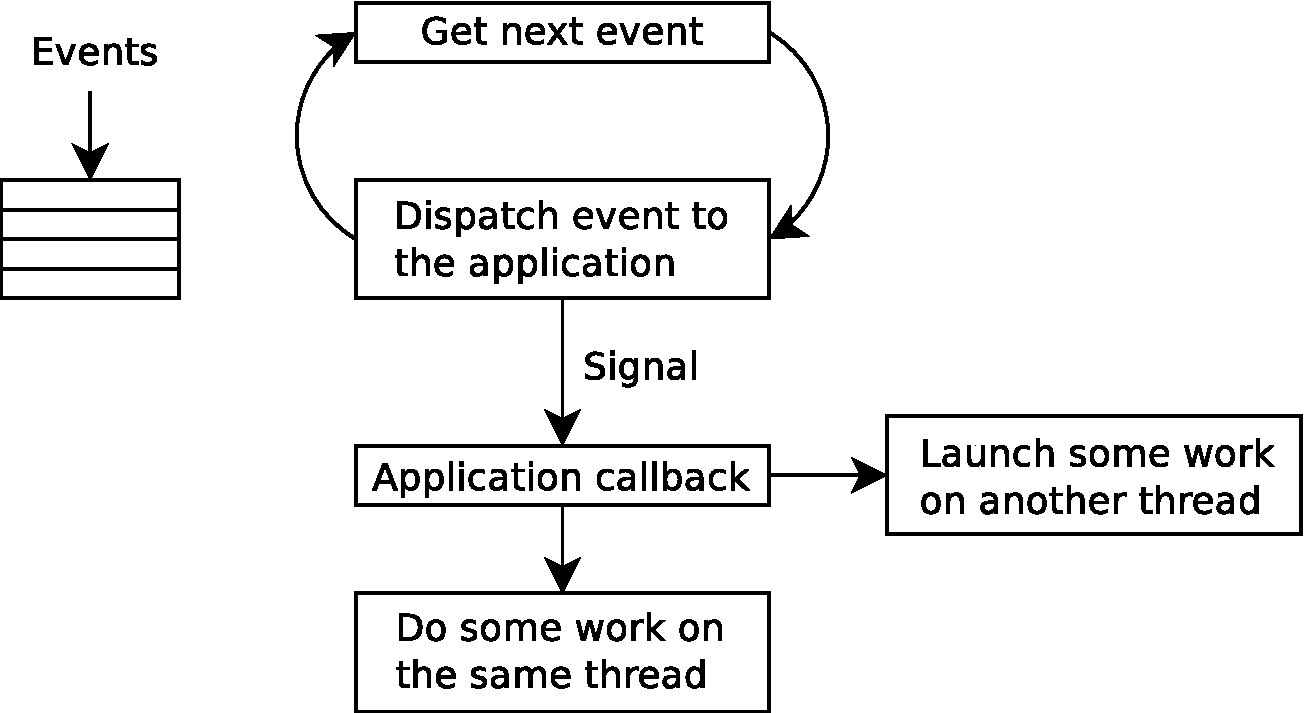
\includegraphics[width=10cm]{assets/img/event-loop.pdf}
    \caption{Structure of an event-driven application, with a main event loop}
    \label{glib-event-loop}
  \end{center}
\end{figure}

Las aplicaciones actuales a menudo se basan en eventos. Para las aplicaciones GUI, hay muchas fuentes de eventos: una pulsación de tecla, un clic del mouse, un gesto táctil, un mensaje de otra aplicación, un cambio en el sistema de archivos, estar conectado o desconectado de la red, etc. Una aplicación necesita reaccionar a esos eventos. Por ejemplo, cuando se presiona una tecla cuando una entrada de texto tiene el foco, el carácter debe insertarse y mostrarse en la pantalla.

Pero la programación dirigida por eventos también se aplica a los demonios. La comunicación entre procesos también ocurre entre daemons y aplicaciones. Un demonio podría recibir un evento cuando llega un paquete a una interfaz de red. Un demonio de impresora podría recibir eventos cuando una impresora está conectada, desconectada, tiene poco papel, etc. Un demonio de montaje puede escuchar las memorias USB insertadas. Otro demonio puede escuchar las conexiones de monitores externos para reconfigurar las pantallas, y así sucesivamente.

Un programa impulsado por eventos no está estructurado de la misma manera que un programa por lotes. El trabajo a realizar por un programa por lotes se determina al principio. Luego analiza la entrada, realiza algunos cálculos sobre ella y genera un informe. Por ejemplo, la mayoría de los comandos y scripts de Unix son programas por lotes.

Entonces, ¿cómo estructurar una aplicación que necesita responder a varios eventos que pueden llegar en cualquier momento? Como sugiere el título de esta sección ... ¡con un \emph{bucle de evento principal} por supuesto! Esa es otra parte importante de GLib; Proporciona soporte básico de programación dirigida por eventos, con una abstracción de bucle de eventos principal, una implementación portátil de subprocesos y comunicación asincrónica entre subprocesos. Un bucle de eventos escucha algunas fuentes de eventos. Se asocia una prioridad con cada fuente de eventos. Cuando llega un evento, el bucle de eventos lo envía a la aplicación. El evento se puede tener en cuenta, ya sea en el mismo hilo o en otro hilo. La Figura~\ref{glib-event-loop} muestra una vista de alto nivel de lo que es un bucle de eventos principal.

La función \lstinline{main()} de una aplicación dirigida por eventos se ve así:
\begin{lstlisting}
gint
main (gint   argc,
      gchar *argv[])
{
  /* Create main window and attach signal callbacks. */

  /* Run the main event loop. */
  gtk_main ();

  return 0;
}
\end{lstlisting}

El bucle de eventos GTK tiene un nivel ligeramente más alto que la abstracción del bucle de eventos GLib. \lstinline{gtk_main()} ejecuta el ciclo de eventos principal hasta que se llama a \lstinline{gtk_main_quit()}. \lstinline{gtk_main_quit()} normalmente se llama en la devolución de llamada de la función cuando se hace clic en el botón de cierre o se activa la acción del menú Salir.

Una devolución de llamada es una función que se llama cuando se envía una señal. El sistema de señales está implementado por la biblioteca GObject. La escucha de una señal se logra con la función \lstinline{g_signal_connect()}:
\begin{lstlisting}
static void
button_clicked_cb (GtkButton *button,
                   gpointer   user_data)
{
  MyObject *self = user_data;

  /* Do something */
}

static void
create_button (MyObject *self)
{
  GtkButton *button;

  /* Create button */

  /* Attach signal callback */
  g_signal_connect (button,
                    "clicked",
                    G_CALLBACK (button_clicked_cb),
                    self);
}
\end{lstlisting}

Cuando se ejecuta una devolución de llamada, bloquea el bucle principal. Entonces, para no congelar la interfaz de usuario, existen dos soluciones:
\begin{enumerate}
    \item Las operaciones largas (especialmente las E/S) se pueden iniciar en otro hilo.
    \item Las operaciones largas se pueden dividir en fragmentos más pequeños, y cada fragmento se ejecuta en una iteración de bucle principal separada.
\end{enumerate}

Para la segunda solución, GLib proporciona las funciones \lstinline{g_idle_add()} y \lstinline{g_timeout_add()} (ver Listado~\ref{glib-idle-timeout}). Se llamará a una función inactiva cuando el bucle principal esté inactivo, es decir, cuando el bucle principal no tenga nada más que hacer. Se llama a una función de tiempo de espera a intervalos regulares. El valor de retorno booleano de una \lstinline{GSourceFunc} permite continuar o detener la función. Si continúa, el bucle principal volverá a llamar a la función en el siguiente tiempo de inactividad o tiempo de espera. Puede eliminar manualmente \lstinline{GSourceFunc} llamando a \lstinline{g_source_remove()}, que toma como parámetro el ID de origen devuelto por \lstinline{g_idle_add()} o \lstinline{g_timeout_add()}. Debe prestar atención para eliminar una \lstinline{GSourceFunc} cuando se destruye el objeto en el que realiza el cálculo. Por lo tanto, puede almacenar el ID de fuente en un atributo de objeto y llamar a \lstinline{g_source_remove()} en el destructor si el ID de fuente es diferente de \lstinline{0}. (Consulte la biblioteca de GObject para crear sus propias clases en C.)

\begin{lstlisting}[float, caption={Inactivos y tiempos de espera}, label=glib-idle-timeout]
#include <glib.h>

typedef gboolean (* GSourceFunc) (gpointer user_data);

guint g_idle_add (GSourceFunc function, gpointer data);
guint g_timeout_add (guint interval, GSourceFunc function, gpointer data);

gboolean g_source_remove (guint source_id);
\end{lstlisting}

\section{Otras características}

Simplemente no hay espacio para cubrir todas las funciones de GLib en este libro. Vale la pena mirar GLib cada vez que piense: ``Realmente \emph{debería} haber una función que ...''. Esta sección enumera otras características que proporciona GLib, pero \emph{no} es exhaustiva.

Parte del soporte de aplicaciones principales que no se ha mencionado aún:
\begin{itemize}
    \item \lstinline{GError}: un sistema de notificación de errores, similar a las excepciones en otros idiomas.
    \item La función \lstinline{g_log ()} le permite imprimir advertencias, mensajes, etc. con niveles de registro configurables y rutinas de impresión conectables.
\end{itemize}

Utilidades:
\begin{itemize}
    \item Un analizador de opciones de línea de comandos.
    \item Un marco de prueba unitaria.
    \item Una instalación de temporizador.
    \item Funciones calendáricas/aritméticas de fechas.
    \item Filename manipulation, such as \lstinline{g_path_get_basename()} and \lstinline{g_path_is_absolute()}.
    \item Un analizador XML simple.
    \item Expresiones regulares compatibles con Perl.
\end{itemize}

Una selección de utilidades más pequeñas:
\begin{itemize}
    \item \lstinline{G_MAXFLOAT}, etc. equivalentes para muchos tipos numéricos.
    \item Conversiones por orden de bytes.
    \item \lstinline{G_DIR_SEPARATOR} maneja las diferencias de Windows/Unix.
    \item Rutinas de conveniencia/portabilidad para obtener el directorio de inicio del usuario, obtener el nombre de un directorio \path{/tmp} y tareas similares.
    \item \lstinline{G_VA_COPY} copia una \lstinline{va_list} de forma portátil.
    \item Numerosas macros para permitir el uso de extensiones del compilador (especialmente extensiones GCC) de forma portátil.
    \item Manipulación de campo de bits.
    \item Portable \lstinline {g_htonl()} y otras conversiones de host a red.
\end{itemize}

Y por último, pero no menos importante, otros tipos de datos interesantes:
\begin{itemize}
    \item Clases mejoradas de cadenas y matrices. Arreglos de punteros y bytes.
    \item \lstinline{GQuark} -- mapeo bidireccional de cadenas a identificadores enteros.
    \item \lstinline{GVariant} -- un tipo de datos genérico que almacena un valor junto con información sobre el tipo de ese valor.
\end{itemize}